\begin{frame}[allowframebreaks]{Fundamentals of Instance Discrimination}
    \textbf{Instance Discrimination} is a self-supervised learning approach where each individual sample in the dataset is treated as a distinct class.
    \begin{itemize}
        \item The core idea is to learn representations by distinguishing between different instances, rather than relying on human-annotated labels.
        \item \textbf{Positive pairs} are generated by applying different augmentations (such as cropping, color jittering, or flipping) to the same image. These augmented views are considered to belong to the same class (i.e., the same instance).
        \item \textbf{Negative pairs} are formed by pairing augmented views of different images. These are treated as belonging to different classes (i.e., different instances).
    \end{itemize}

    \framebreak
    \begin{figure}
        \centering
        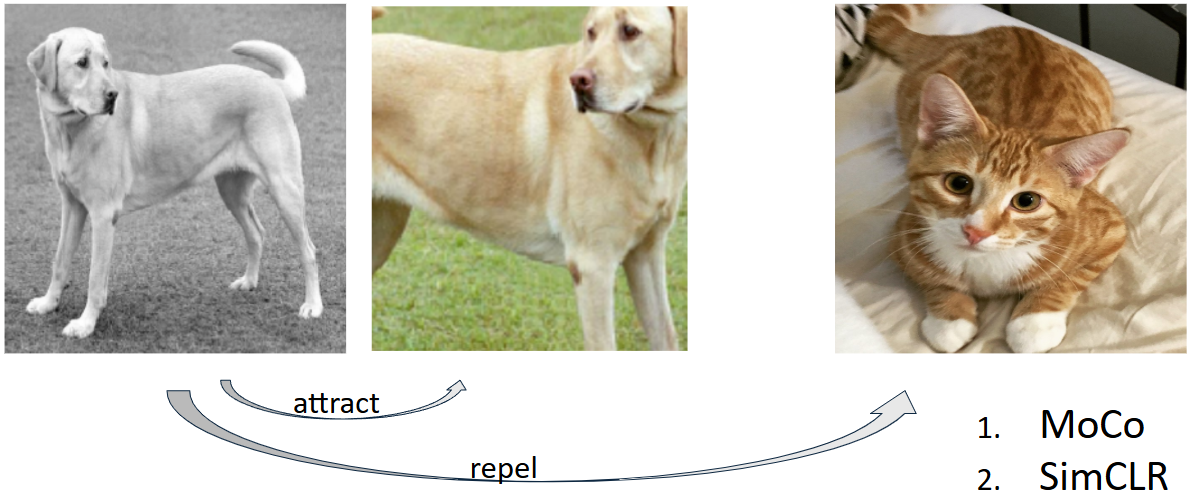
\includegraphics[width=1\linewidth,height=0.9\textheight,keepaspectratio]{images/ssl/slide_63_img.png}
        % \footnote{Wu et al (2018). Unsupervised Feature Learning via Non-Parametric Instance Discrimination. CVPR 2018.}
    \end{figure}

    \framebreak
    \begin{itemize}
        \item The learning objective is to \textbf{maximize agreement} (similarity) between representations of positive pairs, while minimizing agreement between negative pairs.
        \item This is typically achieved using a contrastive loss function, such as InfoNCE, which encourages the model to bring positive pairs closer in the embedding space and push negative pairs apart.
        \item Instance discrimination forms the basis for many popular self-supervised learning methods, such as MoCo, SimCLR, and PIRL.
        \item By maximizing agreement across views of the same instance, the model learns to extract meaningful and invariant features, which can be transferred to downstream tasks.
    \end{itemize}
\end{frame}